A kiírásban megfogalmazott feladat természetéből következik, hogy idősoros adatokat kell
feldolgozni, elemezni, az adatok alapján modellt építeni, az adatokat és végül magát a GDP-t
előrejelezni.

Idősoros adatokat több, alapvetően különböző megközelítésben lehet elemezni. A módszerek közötti
legalapvetőbb különbség az elemzés alapja:
\begin{itemize}
    \item idő
    \item frekvencia
\end{itemize}

\section{Frekvenciavizsgálat alapja és lehetőségei}

Természetesen igaz az alapvető összefüggés:
\begin{equation}
    f = \frac{1}{T}
\end{equation}
ahol $f$ a frekvencia és $T$ a periódus. Azaz az idő és a frekvencia egymás reciprokai.

Fontos még megjegyezni, hogy T periódusidőnek állandónak kell lennie, így önmagában nem elég, ha
csak hétköznapokról van adatunk és a hétvégéről nincs. Pontosabban fogalmazva a
frekvenciatartománybeli vizsgálathoz még felül kell valamilyen módszerrel mintavételezni a mintát.

A frekvencia elemzés fontos sarokköve, hogy minden periodikus jel/minta felírható szinuszon
komponensek szuperpozíciójaként.

Továbbmenve a Nyquist-Shannon-féle mintavételezési tétel szerint az előzőekben említett Fourier
transzformáció legmagasabb frekvenciájú komponensének legalább kétszeresével kell mintavételezni,
ahhoz hogy a jel helyreállítható legyen. Erre egy példa lehet, hogy az emberi hallás 20 és 20 ezer
Hz között működik, így egy jó minőségű hangfelvételnek legalább 40 kHz-esnek kell lennie.

\subsection{A magyar elektromos áram fogyasztás frekvenciatartománybeli vizsgálata}

A MAVIR Zrt.\ honlapján teszi közzé a magyar villamosenergia mind az aktuális mind a historikus
fogyasztási adatokat különböző, akár 1 perces mintavételi idővel. Az adatok, amelyet itt ebben az
esettanulmányban bemutatok, az a 2015.\ január 1.\ éjféltől 2019.\ december 31.\ éjfélig terjedő
időintervallumban mért ``Bruttó hitelesített rendszerterhelése``. A vizsgálódásunknak az a célja,
hogy kimutassuk az elsőre nem feltétlenül látszódó ciklikusságokat.

\begin{figure}[htbp]
    \centering
    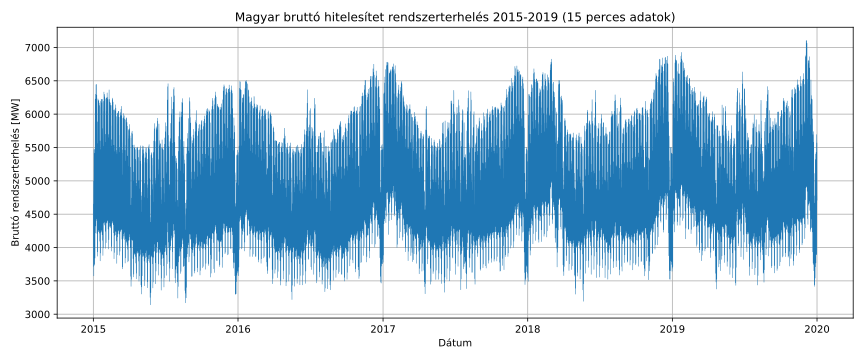
\includegraphics[width=1\textwidth, height=0.8\textheight, keepaspectratio]{../figures/electricity_time.png}
    \caption{Magyar bruttó hitelesítet rendszerterhelés 2015--2019 (15 perces adatok)}\label{fig:electricity_time}
\end{figure}

Előzetesen két periodicitás mindenképp logikusnak tűnik:
\begin{itemize}
    \item Éves periodicitás: a téli fűtési és a nyári légkondicionálási szokások ismétlődése.
    \item Napi periodicitás: a napi rutinok ismétlődése (világítás, fürdővíz).
\end{itemize}

Elvégezve a Fourier transzformációt és az eredményeket ábrázoljuk a következő diagrammot kapjuk:

\begin{figure}[htbp]
    \centering
    \includegraphics[width=1\textwidth, height=0.8\textheight, keepaspectratio]{../figures/electricity_fourier.png}
    \caption{Magyar bruttó hitelesítet rendszerterhelés 2015--2019 --- Fourier-spektrum felharmonikusai (15 perces adatok)}\label{fig:electricity_fourier}
\end{figure}

Leolvasva az öt legmagasabb értéket az ábráról, a következő frekvenciákat kapjuk:

\begin{itemize}
    \item 1 Hz (24 órás periódusidő): alapvető napi biológiai ritmus
    \item 2 Hz (12 órás periódusidő): reggeli és esti rutinok ismétlődése
    \item 0.142 Hz (168 órás periódusidő): heti ismétlődés a szokásokban (pl.\ hétvégi pihenés)
    \item nullához közel (feltehetőleg 0.0274Hz): éves mintázatok
    \item 4 Hz (6 órás periódusidő): napon belüli leállások (étkezés, műszakváltás)
\end{itemize}

Két megjegyzés:

\begin{itemize}
    \item A konstans tagot az ábra nem tartalmazza.
    \item Az adatok aggregált fogyasztást, tehát a lakosság és az ipar együttes fogyasztását mutatja. Az
          ipari tevékenységek sok esetben aszinkron történnek a lakosságival, amelyre a szolgáltatók
          ösztönözni igyekeznek ügyfeleiket, például kedvezményes éjszakai díjszabással. Ez tompítja a napi
          ingadozásokat és kisebb amplitúdókat eredményez a frekvenciatartományban.
\end{itemize}

Az esettanulmányból is láthatjuk, hogy a frekvenciatartománybeli vizsgálatok rámutathatnak fontos
tudásra a mintával kapcsolatban, ezek közöl is a legfontosabb a periodicitás. Ha ezt a GDP-re
vonatkoztatjuk, akkor rejtett üzleti ciklusokat feldezhetünk fel vele. Akár nagyon rövid, akár sok
éves ciklusokat.

Azonban a frekvenciatartománybeli vizsgálat több egyéb kérdést is felvet, amelyekből kettőt itt
megemlítek:

\begin{itemize}
    \item hiányzó adatok az adatsorban
    \item nehezen kezelhetők a gazdasági és politikai válságok hatásai
\end{itemize}

\section{Idősoros vizsgálati módszerek}

\subsection{OLS --- Ordinary Least Square modellek}

\subsection{ETS --- Error, Trend and Seasonality modellek}
Exponenciális simítás

\section{ARMA modellcsalád}

Mielőtt a modellcsalád bemutatásába belekezdek érdemes megismerkedni a \emph{stacionaritás}
fogalmával. Azt mondjuk, hogy egy idősoros adat \emph{stacionárius}, ha

\begin{itemize}
    \item az átlaga konstans
    \item a szórása konstans
    \item a sokaságon belüli autokorrelációk is konstansak
\end{itemize}

\subsection{Augmented Dickey–Fuller teszt (ADF)}

\subsection{AR --- Autoregresszív modellek}

A legegyszerűbb autoregresszív modell az $AR(1)$ modell:

\begin{equation}
    y_t = a_1y_{t-1} + \epsilon_t
\end{equation}

A zárójelben szereplő 1-es azt fejezi ki, hogy az $y$ mostani értéke az $y$ előző érték $a_1$
szorosa, amelyre egy hibataga $\epsilon_t$ tevődik, amely fehérzajnak feleltethető meg.

Eggyel továbblépve a másodrendű autóregresszív modell az $AR(2)$:

\begin{equation}
    y_t = a_1y_{t-1} + a_2y_{t-2} + \epsilon_t
\end{equation}

Általánosítva a modellt, kapjuk a p-rendű $AR(p)$ modellt:

\begin{equation}
    y_t = a_1y_{t-1} + a_2y_{t-2} + \ldots + a_p y_{t-p} + \epsilon_t % chktex 11
\end{equation}

\subsection{MA --- Moving Average modellek}

Mozgóátlag modellek hasonlítanak az autoregresszív modellekhez, viszont itt a modell $m_i$
paraméterei nem az előző értékre, hanem az előző hibatagra vonatkoznak. Az így kapott modell az
$MA(1)$ modell:

\begin{equation}
    y_t = m_1\epsilon_{t-1} + \epsilon_t
\end{equation}

Általánosítva kapjuk $MA(q)$ modellt, ahol $q$ a modell rendje:

\begin{equation}
    y_t = m_1\epsilon_{t-1} + m_2\epsilon_{t-2} + \ldots + m_q\epsilon_{t-q} + \epsilon_t % chktex 11
\end{equation}

\subsection{ARMA --- AR+MA modellek}

Az ARMA modell az autóregresszív és mozgóátlagon alapuló modellek kombinációja. Az $ARMA(1,1)$
modellt tehát a következő képlet ír le:

\begin{equation}
    y_t = a_1y_{t-1} + m_1\epsilon_{t-1} + \epsilon_t
\end{equation}

A fenti képletet általánosítva kapjuk az $ARMA(p,q)$ modellt, ahol $p$ az autoregresszív rész
rendje és $q$ a mozgóátlagos rész rendje:

\begin{equation}
    y_t = a_1y_{t-1} + a_2y_{t-2} + \ldots + a_p y_{t-p} + m_1\epsilon_{t-1} + m_2\epsilon_{t-2} + \ldots + m_q\epsilon_{t-q} + \epsilon_t % chktex 11
\end{equation}

\subsection{ARMAX --- ARMA modellek exogén változókkal kiegészítve}

Itt már csak az elsőrendű alakot, az $ARMAX(1,1)$ modellt hozom, ahol $x$ az exogén változó és
$z_1$ annak a koefficiense:

\begin{equation}
    y_t = z_1x_t + a_1y_{t-1} + m_1\epsilon_{t-1} + \epsilon_t
\end{equation}

\subsection{ARIMA --- Az integráló ARMA modellek}
\subsection{SARIMA --- Seasonal ARIMA modellek}

Sok esetben

\begin{equation}
    y_t = z_1x_t + a_1y_{t-1} + m_1\epsilon_{t-1} + \epsilon_t
\end{equation}

\subsection{ML --- Machine Learning modellek}

\section{Projektfeladatban alkalmazott modellek}